\documentclass[twocolumn]{aastex63}


\usepackage{graphicx}	% Including figure files



\newcommand{\vdag}{(v)^\dagger}
\newcommand\aastex{AAS\TeX}
\newcommand\latex{La\TeX}

\newcommand{\eduardo}[1]{{\color{teal}E: #1}}
\newcommand{\jorge}[1]{{\color{magenta}J: #1}}
\newcommand{\cesar}[1]{{\color{red}C: #1}}
\newcommand{\Karla}[1]{{\color{violet}K: #1}}
%% Reintroduced the \received and \accepted commands from AASTeX v5.2
\received{XXX}
\revised{YYY}
\accepted{ZZZ}
%% Command to document which AAS Journal the manuscript was submitted to.
%% Adds "Submitted to " the argument.
\submitjournal{ApJ}
\shortauthors{M\'endez-Delgado et al.}

\graphicspath{{./}{figures/}}
%% This is the end of the preamble.  Indicate the beginning of the
%% manuscript itself with \begin{document}.


\begin{document}

\title{Photoionized Herbig-Haro objects in the Orion Nebula through deep high-spectral resolution spectroscopy II: HH~204}


\shorttitle{HH~204 in the Orion Nebula}



\correspondingauthor{Jos\'e E. M\'endez-Delgado}
\email{jemd@iac.es}

\author[0000-0002-6972-6411]{J. E. M\'endez-Delgado}
\affiliation{Instituto de Astrof\'isica de Canarias (IAC), E-38205 La Laguna, Spain}
\affiliation{Departamento de Astrof\'isica, Universidad de La Laguna, E-38206 La Laguna, Spain}


\author[0000-0002-5247-5943]{C. Esteban}
\affiliation{Instituto de Astrof\'isica de Canarias (IAC), E-38205 La Laguna, Spain}
\affiliation{Departamento de Astrof\'isica, Universidad de La Laguna, E-38206 La Laguna, Spain}


\author[0000-0002-6138-1869]{J. Garc\'ia-Rojas}
\affiliation{Instituto de Astrof\'isica de Canarias (IAC), E-38205 La Laguna, Spain}
\affiliation{Departamento de Astrof\'isica, Universidad de La Laguna, E-38206 La Laguna, Spain}


\author[0000-0001-6208-9109]{W. J. Henney}
\affiliation{Instituto de Radioastronom\'ia y Astrof\'isica, Universidad Nacional Aut\'onoma de M\'exico, Apartado Postal 3-72, 58090 Morelia, Michoac\'an, Mexico}

\author[0000-0003-3776-6977]{A. Mesa-Delgado}
\affiliation{Calle Camino Real 64, Icod el Alto, Los Realejos, 38414, Tenerife, Spain}

\author[0000-0002-2644-3518]{K. Z. Arellano-C\'ordova}
\affiliation{The University of Texas at Austin, 2515 Speedway Boulevard Stop C1400, Austin, TX 78712, USA}


\received{XXX}
\revised{YYY}
\accepted{ZZZ}

%\nocollaboration{1}



%\collaboration{1}{(LaTeX collaboration)}

%\nocollaboration{2}

%% Note that the \and command from previous versions of AASTeX is now
%% depreciated in this version as it is no longer necessary. AASTeX 
%% automatically takes care of all commas and "and"s between authors names.

%% AASTeX 6.3 has the new \collaboration and \nocollaboration commands to
%% provide the collaboration status of a group of authors. These commands 
%% can be used either before or after the list of corresponding authors. The
%% argument for \collaboration is the collaboration identifier. Authors are
%% encouraged to surround collaboration identifiers with ()s. The 
%% \nocollaboration command takes no argument and exists to indicate that
%% the nearby authors are not part of surrounding collaborations.

%% Mark off the abstract in the ``abstract'' environment. 
\begin{abstract}

Contribuciones de Will para el artículo

\end{abstract}

%% Keywords should appear after the \end{abstract} command. 
%% See the online documentation for the full list of available subject
%% keywords and the rules for their use.
\keywords{ISM:Abundances – ISM: Herbig–Haro objects – ISM: individual:
Orion Nebula – ISM: individual: HH 204}

\section{Material de Will}
\label{sec:will}

\newcommand\ha{\ensuremath{\mathrm{H\alpha}}}
\newcommand\hb{\ensuremath{\mathrm{H\beta}}}
% aastex \ion command is useless - must replace it
\newcounter{ionstage}
\renewcommand{\ion}[2]{\setcounter{ionstage}{#2}% 
  \ensuremath{\mathrm{#1\,\scriptstyle\Roman{ionstage}}}}
\newcommand\oiii{[\ion{O}{3}]}
\newcommand\wav[1]{\ensuremath{\lambda #1}}
% Stars in Orion, e.g., \th1C, \th2A
\def\th#1#2{\ensuremath{\theta^{#1}\,\text{Ori~#2}}}

\begin{figure*}
  \centering
  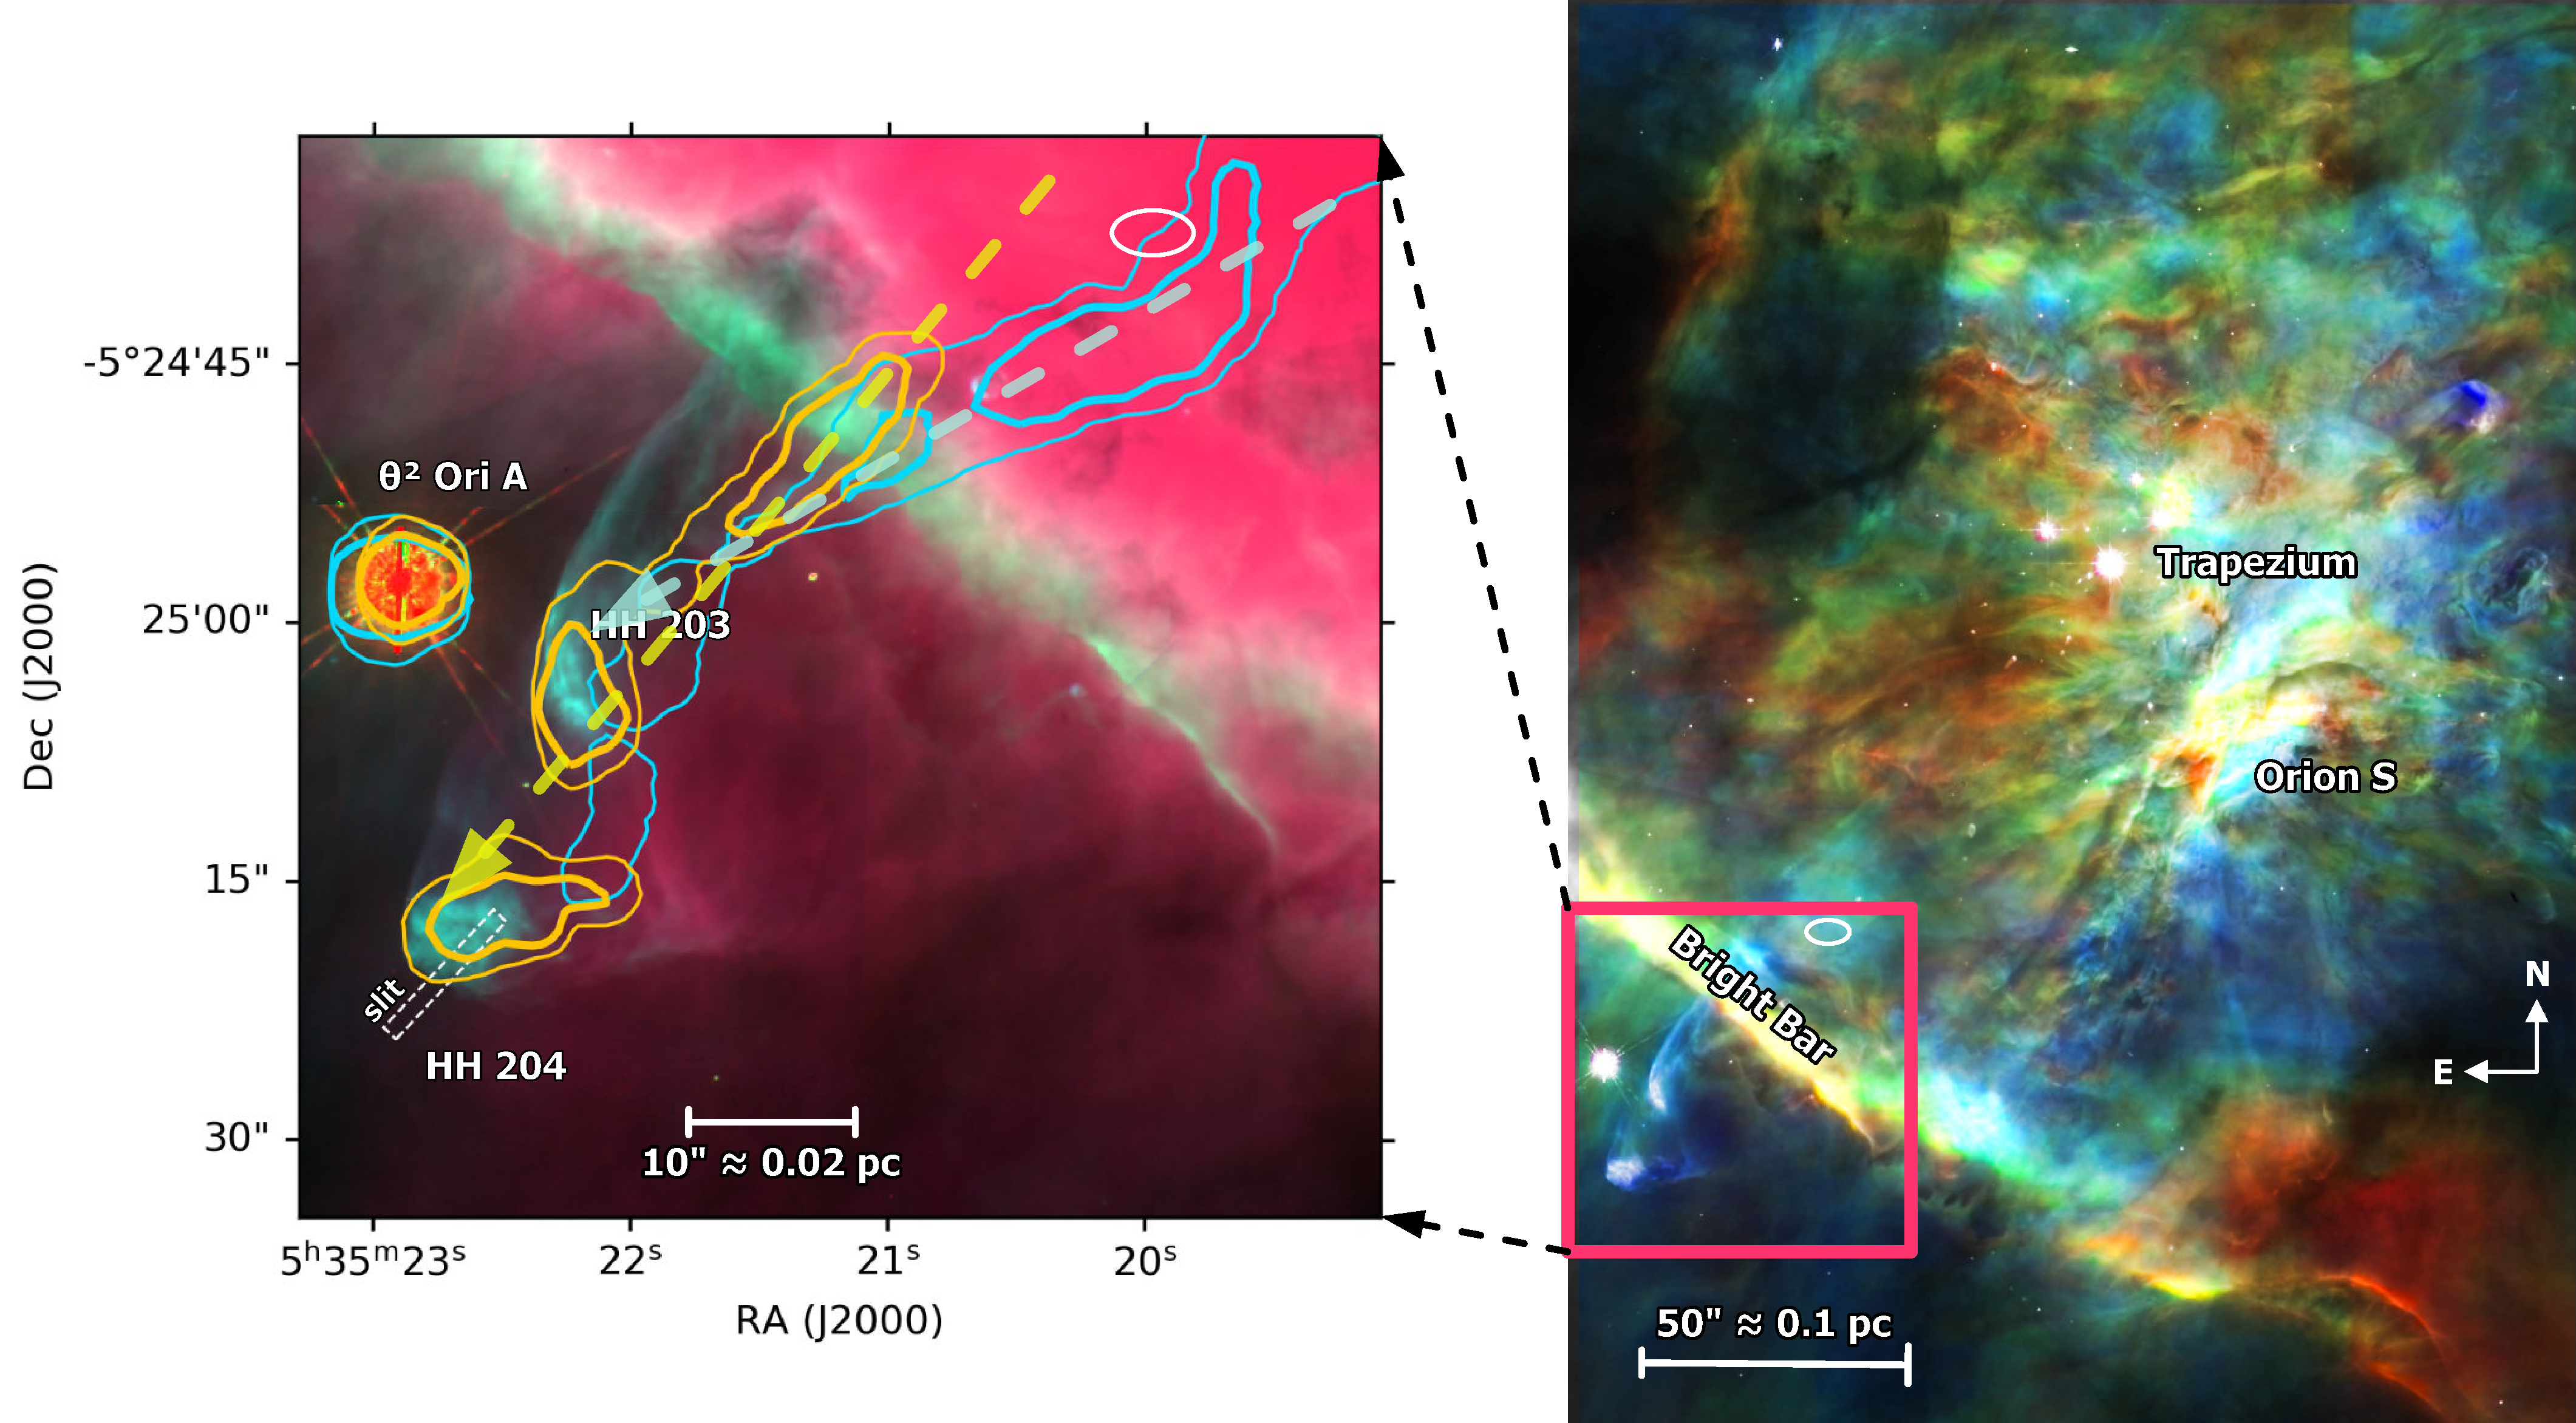
\includegraphics[width=\textwidth]{hh204-finding-chart}
  \caption{Finding chart.}
  \label{fig:hh204-finding-chart}
\end{figure*}


\begin{figure}
  \centering
  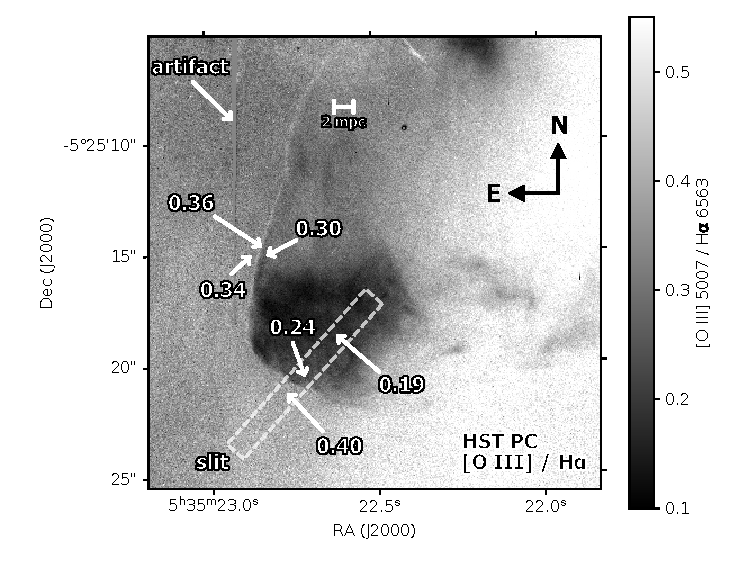
\includegraphics[width=\columnwidth]{hh204-ratio-oiii-ha-annotated}
  \caption{
    Map of the line ratio \(\oiii{}\ \wav{5007} / \ha\ \wav{6563}\),
    calculated from \textit{HST} images with the PC chip of the WFPC2 camera.
    Particular values of interest are indicated by arrows.
    The position of the UVES spectrograph slit is outlined by dashed lines.
    The vertically oriented ``scar'' at upper left is an artifact
    due to the bright star \th2A, located just north of the field of view.}
  \label{fig:ratio-hst-oiii-ha}
\end{figure}


\subsection{Sub-arcsecond imaging of HH 204}
\label{sec:high-resol-imag}

Figure~\ref{fig:ratio-hst-oiii-ha} shows the ratio of surface brightnesses
\(\oiii\ \wav{5007} / \ha\ \wav{6563}\) calculated from \textit{HST} WFPC2
observations in the F502N, F547M, F656N, and F658N filters
from program GO5469 \citep{ODell:1996a}.
Flux calibration and correction for contamination by continuum and non-target lines
was performed using the coefficients given in \citet{ODell:2009b}.
It can be seen that the line ratio in the background nebula shows a pronounced gradient
from \(\wav{5007} / \ha \approx 0.3\) in the north-east
to \(\wav{5007} / \ha \approx 0.5\) in the south-west.%
\footnote{
  For comparison with results from our UVES spectra,
  and using the average reddening for the HH~204 region \citep{Weilbacher:2015a},
  the conversion is \(\wav{4959} / \hb \approx 1.1 \wav{5007} / \ha\).
}
Inside the bow shock, the ratio is significantly smaller,
for instance falling from \(\simeq 0.4\) to \(\simeq 0.2\) along the length of the slit. 



\bibliography{will-hh204-refs}


\end{document}
